\documentclass[a4paper,12pt]{article}
\usepackage{geometry}
 \geometry{
 a4paper,
 total={170mm,257mm},
 left=20mm,
 top=20mm,
 }
\usepackage{adjustbox}
\usepackage[polish]{babel}
\usepackage{polski}
\usepackage{multirow}
\usepackage{makecell}
\usepackage{boldline}
\usepackage[T1]{fontenc} 
\usepackage{listings}
\usepackage{color}
\usepackage{biblatex}
\usepackage{csquotes}
\usepackage{indentfirst}
\usepackage{subfig}
\addbibresource{cmake.bib}

\lstset{literate={ą}{{\k{a}}}1 {ł}{{\l{}}}1 {ń}{{\'n}}1 {ę}{{\k{e}}}1 {ś}{{\'s}}1 {ż}{{\.z}}1 {ó}{{\'o}}1 {ź}{{\'z}}1 {Ą}{{\k{A}}}1 {Ł}{{\L{}}}1 {Ń}{{\'N}}1 {Ę}{{\k{E}}}1 {Ś}{{\'S}}1 {Ż}{{\.Z}}1 {Ó}{{\'O}}1 {Ź}{{\'Z}}1 {Ć}{{\'C}}1 {ć}{{\'c}}1 }

\title{Sprawozdanie z Zadania: Zapoznanie się z narzędziami make i cmake}
\author{Jakub Kraus}
\date{24.01.2024}
\renewcommand\theadalign{tl}
\begin{document}
\renewcommand{\arraystretch}{2}
\begin{table}[ht]
    \centering
    \begin{adjustbox}{width=1\textwidth,center=\textwidth}
        \begin{tabular}{V{4}lV{4}c|c|c|c|c|c V{4}}
            \hlineB{4}
            \multicolumn{2}{V{4}lV{4}}{}                                         & \multicolumn{5}{lV{4}}{\textbf{Wydział Nauk Ścisłych i Technicznych}}                                                                                                                                   \\
            \cline{3-7}
            \multicolumn{2}{V{4}cV{4}}{\textbf{Uniwersytet Śląski w Katowicach}} & \multicolumn{5}{lV{4}}{\textbf{Instytut Fizyki}}                                                                                                                                                        \\
            \cline{3-7}
            \multicolumn{2}{V{4}lV{4}}{}                                         & Rok                                                                   & \textbf{III}                                          & Semestr                            & \multicolumn{2}{cV{4}}{\textbf{V}} \\
            \hlineB{4}
            Kierunek                                                             & \multicolumn{6}{cV{4}}{Informatyka stosowana}                                                                                                                                                           \\
            \hline
            Przedmiot                                                            & \multicolumn{6}{cV{4}}{\textbf{SiNWO - laboratorium}}                                                                                                                                                   \\
            \hlineB{4}
            Prowadzący                                                           & \multicolumn{6}{cV{4}}{dr Wojciech Gurdziel}                                                                                                                                                            \\
            \hline
            Tytuł ćwiczenia                                                      & \multicolumn{4}{c|}{\textbf{Wprowadzenie do make i cmake}}            &
            \multirow{2}{*}{Nr ćwiczenia}                                        & \multirow{2}{*}{\textbf{III}}                                                                                                                                                                           \\
            \cline{1-5}
            \thead{Sprawozdanie wykonał:                                                                                                                                                                                                                                                   \\ (Imię i Nazwisko)} &
            \multicolumn{4}{c|}{\textbf{Jakub Kraus}}                            &                                                                       &                                                                                                                                 \\
            \hlineB{3}
            Data wykonania ćwiczenia                                             & \textbf{24.01.2024}                                                   & \multicolumn{2}{V{4}lV{4}}{Data oddania sprawozdania} & \multicolumn{3}{cV{4}}{31.01.2024}                                      \\
            \hlineB{4}
        \end{tabular}
    \end{adjustbox}
\end{table}
\newpage
\tableofcontents
\listoffigures
\newpage
\section{Cel ćwiczenia}
Celem ćwiczenia było zapoznanie się z narzędziami make oraz cmake i ich zastosowaniem w procesie kompilacji programów.
\section{Przebieg ćwiczenia}
Do wykonania ćwiczenia wykorzystałem system operacyjny openSUSE Tumbleweed\cite{noauthor_opensuse_nodate} oraz narzędzie cmake\cite{noauthor_cmake_nodate}.
\subsection{Wybór narzędzia}
W ramach ćwiczenia należało wybrać jedno z narzędzi, które zostaną użyte do kompilacji programów. Wybór padł na narzędzie \textbf{cmake}, ponieważ jest ono bardziej rozbudowane i pozwala na automatyzację procesu kompilacji.
\subsection{Przygotowanie środowiska}
W celu przygotowania środowiska należało zainstalować narzędzie cmake. W tym celu należało wykonać polecenie:
\begin{lstlisting}[language=bash]
    sudo zypper install cmake
\end{lstlisting}
oraz kompilator języka \verb!C++!:
\begin{lstlisting}[language=bash]
    sudo zypper install gcc-c++
\end{lstlisting}


\subsection{Przygotowanie plików źródłowych \texttt{C++}}
W celu przetestowania działania narzędzia cmake przygotowałem pliki źródłowe programu w języku \verb!C++!.
\begin{figure}[ht]
    \centering
    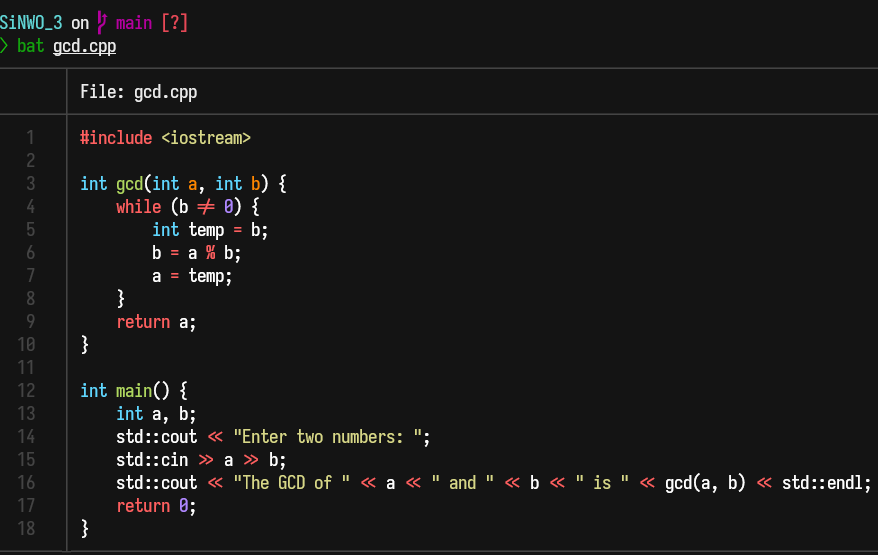
\includegraphics[width=0.8\textwidth]{images/code.png}
    \caption{Zawartość pliku gcd.cpp}
\end{figure}

\newpage
\clearpage

\subsection{Przygotowanie pliku CMakeLists.txt}
W celu kompilacji programu należało przygotować plik \verb!CMakeLists.txt!.
\begin{figure}[ht]
    \centering
    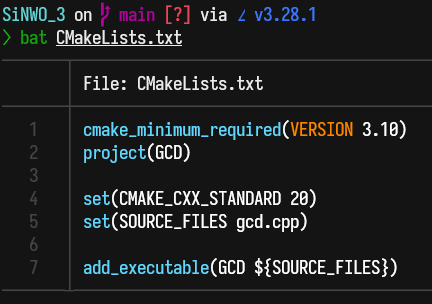
\includegraphics[width=0.6\textwidth]{images/cmake.png}
    \caption{Plik CMakeLists.txt}
\end{figure}

\subsection{Generowanie plików budujących}
W celu wygenerowania plików budujących należało stworzyć folder docelowy i wykonać polecenie:
\begin{figure}[ht]
    \centering
    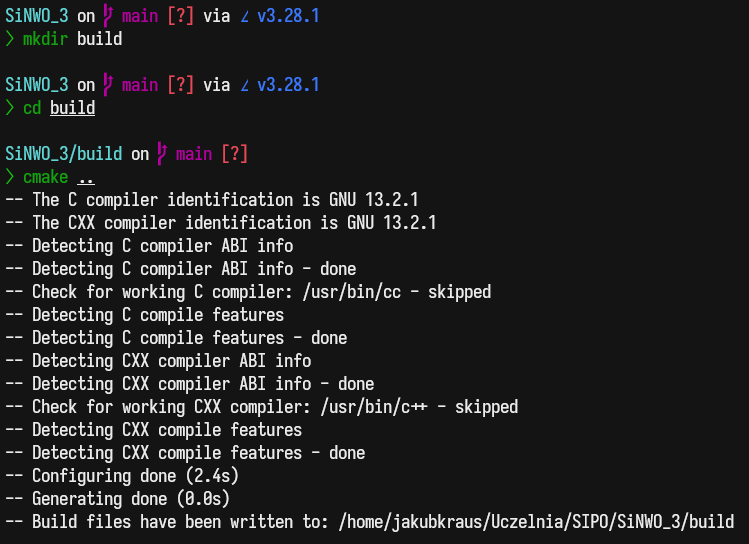
\includegraphics[width=0.8\textwidth]{images/gnu-build.png}
    \caption{Tworzenie folderu i plików budujących}
\end{figure}

\newpage
\clearpage

\subsection{Kompilacja programu i uruchomienie}
W celu kompilacji programu należało wykonać polecenie:
\begin{figure}[ht]
    \centering
    \subfloat[Cmake build i zawartość katalogu build]{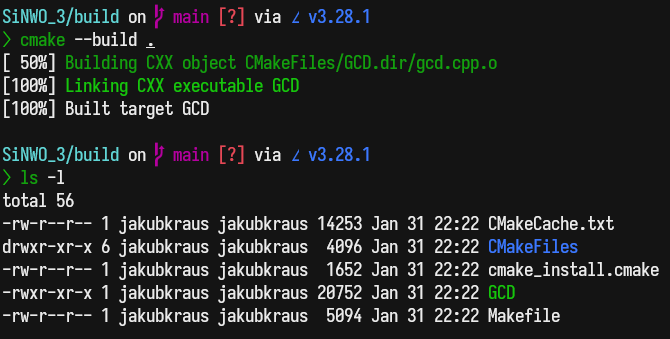
\includegraphics[width=0.8\textwidth]{images/buildowanie.png}}
    \vfill
    \subfloat[Uruchomienie programu]{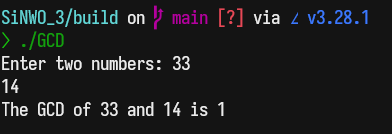
\includegraphics[width=0.5\textwidth]{images/run-built.png}}
    \caption{Utworzenie plików wykonywalnych i uruchomienie programu}
\end{figure}

\newpage
\clearpage

\section{Wnioski}
CMake dostarcza narzędzie do konfiguracji, kompilacji i instalacji projektów w sposób niezależny od platformy. Możliwość definiowania projektów w sposób zależny od platformy pozwala na przenośność kodu między różnymi systemami operacyjnymi. Dzięki CMake i narzędziom kompilacyjnym, takim jak Make, możliwa jest automatyzacja procesu kompilacji. Po skonfigurowaniu projektu za pomocą CMake, polecenie \begin{lstlisting}
    cmake --build .
\end{lstlisting} pozwala na skompilowanie projektu bez konieczności ręcznego zarządzania szczegółami kompilacji. CMake umożliwia integrację testów w proces budowy projektu za pomocą polecenia ctest. Ponadto, opcja \begin{lstlisting}
    cmake --install .
\end{lstlisting} pozwala na instalację skompilowanego projektu na systemie, co może być przydatne w przypadku rozpowszechniania gotowych aplikacji.
\vskip 0.5cm
Podsumowując, CMake stanowi skuteczne narzędzie do zarządzania procesem kompilacji, które oferuje wiele możliwości konfiguracyjnych i ułatwia tworzenie projektów w języku C++ (a także w innych językach programowania).
\printbibliography
\nocite{*}
\end{document}